% Chapter discussion

\chapter{Aim of the study} % Main chapter title

\label{Chapter2} % For referencing the chapter elsewhere, use \ref{Chapter4} 

%----------------------------------------------------------------------------------------

% Define some commands to keep the formatting separated from the content 
\newcommand{\keyword}[1]{\textbf{#1}}
\newcommand{\tabhead}[1]{\textbf{#1}}
\newcommand{\code}[1]{\texttt{#1}}
\newcommand{\file}[1]{\texttt{\bfseries#1}}
\newcommand{\option}[1]{\texttt{\itshape#1}}

%~~~~~~~~~~~~~~~~~~~~~~~~~~~~~~~~~~~~~~~~~~~~~~~~~~~~~~~~~~~~~~~~~~~~~~~~~~~~~~~~~~~~~~~

%~~~~ aim:
The aim of this study is to identify genomic variants likely to cause idiopathic pregnancy losses that are not seen by current diagnostic tools either because of their very small size or because they lie in non-coding regulatory regions of the genome that are not routinely sequenced.

The expectation is to identify highly deleterious dominant \textit{de novo} mutations in sporadic cases and rare moderately deleterious recessive mutations in homozygosis or compound heterozygosity in recurrent pregnancy losses (Figure \ref{fig:expectation}).\\

%~~~~ objectives: 
The objectives were to: 

- analyze whole-genome sequencing data to assemble human sequences obtained by sequencing of miscarried embryos and identify genomic variants

- develop a pipeline to prioritize genetic variants based on their putative deleteriousness  

- identify diagnostic mutations\\

%~~~~ novelties: 
There are two main novelties in this study. First, compared to previous studies, it investigates the genome of the embryos rather than those of parents. Secondly, it uses a whole-genome approach, through high-coverage (30X) whole-genome sequencing allowing to investigate not only genic regions but also regulatory and intergenic ones.

\begin{figure}[H]
\centering
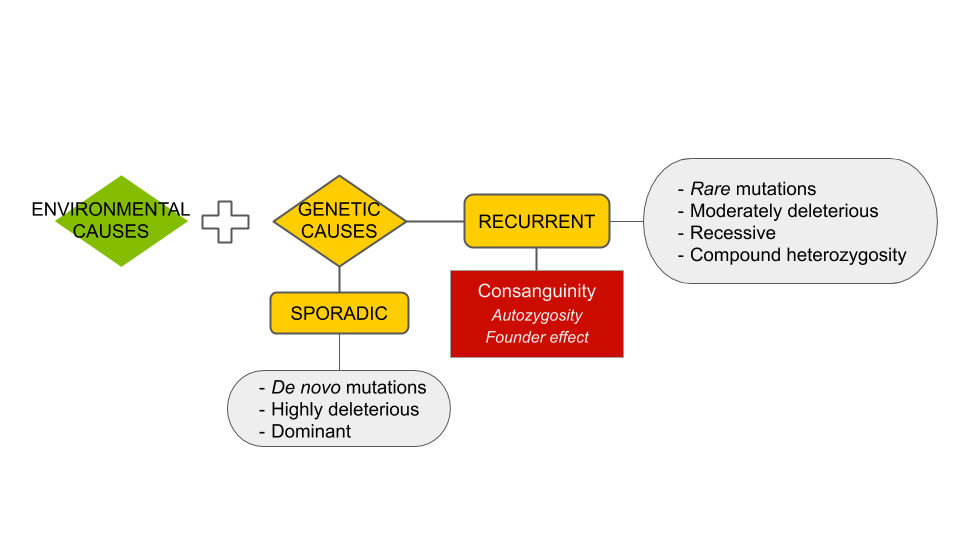
\includegraphics[width=0.90\textwidth]{fig/expectation.png}
\decoRule
\caption{\textbf{Genetic model behind miscarriages.} Expectations on types and frequencies of mutations.} 
\label{fig:expectation}
\end{figure}